\documentclass[../../main.tex]{subfiles}
\graphicspath{{../../image/}{../../figure/}}
\begin{document}

\section{一个非齐次守恒律}\label{section:ch11-一个非齐次守恒律}

这里讨论非齐次守恒律
\begin{align}
\partial_t u(x,t)+\partial_x f(u(x,t),x)=0\label{align:ch11-11-11-1}
\end{align}
的周期解的大时间行为, 其中 $f$ 是 $C^2$ 函数, 满足如下性质:

(a) 关于 $x$ 周期: $f(u,x+1)=f(u,x)$, $-\infty<u<\infty$, $-\infty<x<\infty$。

(b) 真正非线性: $f_{uu}(u,x)\geqslant\mu>0$, $-\infty<u<\infty$, $-\infty<x<\infty$。

(c) 临界点集由极小点与鞍点组成。存在 $\bar u\in(-\infty,\infty)$, $b\in(0,1)$, $x_k=b+k$, $k=0,\pm1,\pm2,\cdots$, 满足: $f_u(\bar u,x_k)=f_x(\bar u,x_k)=0$, $f_{uu}(\bar u,x_k)f_{xx}(\bar u,x_k)-f_{ux}^2(\bar u,x_k)>0$; 并且 $f_u(0,k)=f_x(0,k)=0$, $f_{uu}(0,k)f_{xx}(0,k)-f_{ux}^2(0,k)<0$。

(d) 归一化: $f(0,k)=0$, 因而 $f(\bar u,x_k)<0$。

此类函数的典型例子是 $f(u,x)=u^2-\sin^2(\pi x)$。

对无激波特征线, 系统\eqref{align:ch11-11-9-8}此处取形式
\begin{align}
\begin{cases}
\dot{\xi}=f_u(v,\xi)\\
\dot{v}=-f_x(v,\xi).
\end{cases}\label{align:ch11-11-11-2}
\end{align}

如\cref{chapter:ch11-一维标量守恒律}所述, \eqref{align:ch11-11-11-2}的轨道是函数 $f(u,x)$ 的水平曲线。由 $f$ 的性质, \eqref{align:ch11-11-11-2}的相图如\cref{figure:ch11-11-11-1}所示。在水平曲线 $f=p$ 上, $p>0$ 的轨道是单向的, 从左到右或从右到左。相反, 在水平曲线 $f=p$ 上, $p<0$ 的轨道是周期的。最后, 位于水平曲线 $f=0$ 上的轨道是异宿的, 连接相邻鞍点; 特别地, 位于非负分支 $v=v_+(x)$ 上的轨道连接 $(k+1,0)$ 与 $(k,0)$, 而位于非正分支 $v=v_-(x)$ 上的轨道连接 $(k,0)$ 与 $(k+1,0)$, $k=0,\pm1,\pm2,\cdots$。

\begin{figure}[htbp]
\centering
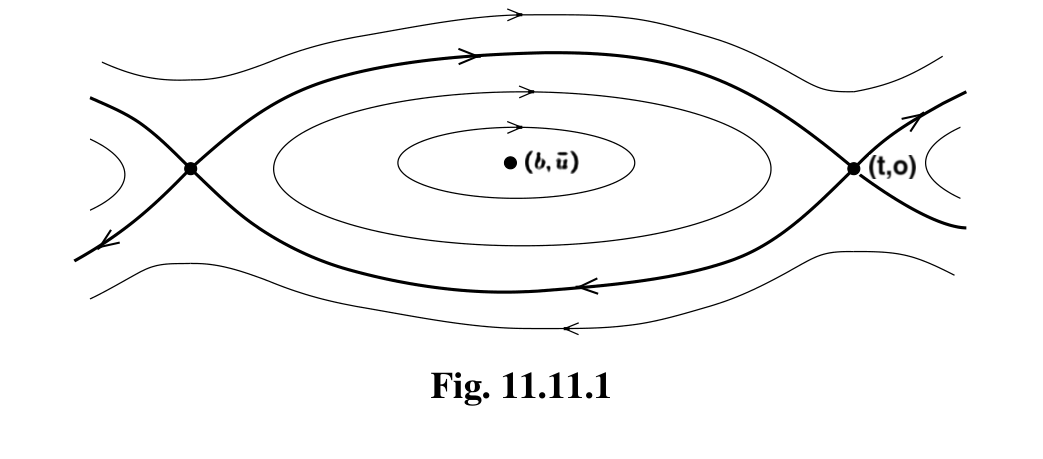
\includegraphics[width=0.7\textwidth]{ch11-fig11-1.png}
\caption{系统\eqref{align:ch11-11-11-2}的相图。}
\label{figure:ch11-11-11-1}
\end{figure}

对 $p\in[f(\bar u,b),\infty)\setminus\{0\}$, 定义 $T(p)$ 如下: 若 $p<0$, $T(p)$ 是绕水平曲线 $f=p$ 的周期。若 $p>0$, $T(p)$ 是沿水平曲线 $f=p$ 穿过长度为二的 $\xi$ 区间所需时间。沿任意轨道流动迅捷, 除在平衡点 $(k,0)$ 附近处减速。在 $(k,0)$ 处线性化系统中, 在平衡点附近逗留时间为 $-\lambda_0^{-1}\log|p|$ 时间单位, 其中 $\pm\lambda_0$ 是向量场 $(f_u,-f_x)$ 的 Jacobi 矩阵在鞍点 $(0,k)$ 处的特征值, 即 $\lambda_0=[f_{ux}^2(k,0)-f_{uu}(k,0)f_{xx}(k,0)]^{1/2}$。因此,
\begin{align}
\frac{T(p)}{\log|p|}=-\frac{2}{\lambda_0}+o(1),\quad p\to0.\label{align:ch11-11-11-3}
\end{align}

对任意 $M\in(-\infty,\infty)$, 方程\eqref{align:ch11-11-11-1}有唯一可容许周期驻波解 $u_M(x)$, 均值为 $M$。令
\begin{align}
M_\pm=\int_0^1 v_\pm(x)\,\mathrm{d}x.\label{align:ch11-11-11-4}
\end{align}

当 $M\geqslant M_+$ 或 $M\leqslant M_-$ 时, $u_M(x)$ 就是均值为 $M$ 的唯一水平曲线 $f=p\geqslant0$。相反, 当 $M_-<M<M_+$ 时, $u_M$ 是弱解, 每个周期含单个可容许驻激波:
\begin{align}
u_M(x)=
\begin{cases}
v_+(x), & k\leqslant x<k+a\\
v_-(x), & k+a<x<k+1,
\end{cases}\quad k=0,\pm1,\pm2,\cdots,\label{align:ch11-11-11-5}
\end{align}
其中 $a\in(0,1)$ 由
\begin{align}
\int_0^a v_+(x)\,\mathrm{d}x+\int_a^1 v_-(x)\,\mathrm{d}x=M.\label{align:ch11-11-11-6}
\end{align}
确定。

目的是证明, 当 $t\to\infty$, 均值为 $M$ 的\eqref{align:ch11-11-11-1}的 1-周期解收敛到 $u_M$。我们仅讨论有趣情形 $M_-<M<M_+$。

\begin{theorem}\label{theorem:ch11-11-11-1}
设 $u(x,t)$ 是\eqref{align:ch11-11-11-1}在上半平面上的可容许解, 初值 $u_0(x)$ 是均值 $M\in(M_-,M_+)$ 的 1-周期函数。则当 $t\to\infty$, 对任意 $\lambda<\lambda_0$,
\begin{align}
f(u(x\pm,t),x)=o\left(e^{-\lambda t}\right),\quad \text{在 }(-\infty,\infty)\text{ 上一致},\label{align:ch11-11-11-7}
\end{align}
\begin{align}
u(x\pm,t)=
\begin{cases}
v_+(x)+o\left(e^{-\frac12\lambda t}\right), & k\leqslant x<\chi_k(t)\\
v_-(x)+o\left(e^{-\frac12\lambda t}\right), & \chi_k(t)<x\leqslant k+1,
\end{cases}\quad k=0,\pm1,\pm2,\cdots,\label{align:ch11-11-11-8}
\end{align}
其中
\begin{align}
\chi_k(t)=k+a+o\left(e^{-\frac12\lambda t}\right),\label{align:ch11-11-11-9}
\end{align}
$a$ 由\eqref{align:ch11-11-11-6}确定。
\end{theorem}

\begin{proof}
固定任意 $k=0,\pm1,\pm2,\cdots$, 注意
\begin{align}
\int_k^{k+1}u(x,t)\,\mathrm{d}x=M.\label{align:ch11-11-11-10}
\end{align}

由于 $M\in(M_-,M_+)$, \eqref{align:ch11-11-11-10} 蕴含存在 $x\in(k,k+1)$ 使 $f(u(x-,t),x)=p<0$。对这样的 $x$, 从点 $(x,t)$ 出发的极小后向特征线 $\zeta(\cdot)$ 是位于水平曲线 $f=p$ 上的 $T(p)$-周期轨道在 $[0,t]$ 上的限制。从点 $(\bar x,t)$ 出发, 其中 $\bar x=x-\varepsilon$, $\varepsilon>0$ 充分小, 极小后向特征线 $\bar\zeta(\cdot)$ 同样是位于某水平曲线 $f=\bar p$, $|p-\bar p|$ 小, 上的周期轨道在 $[0,t]$ 上的限制。

由相图\cref{figure:ch11-11-11-1}, 若 $t$ 大于周期 $T(p)$, 则 $\zeta(\cdot)$ 与 $\bar\zeta(\cdot)$ 的图像必在某时刻 $\tau\in(0,t)$ 相交, 与\cref{theorem:ch11-11-9-4}矛盾。因此 $t\leqslant T(p)$, 从而由\eqref{align:ch11-11-11-3}, $f(u(x-,t),x)\to0$, $t\to\infty$。

接下来假设存在 $x\in[k,k+1]$ 使 $f(u(x-,t),x)=p>0$。固定 $\bar x$ 使 $\bar x<x<\bar x+1$ 且 $f(u(\bar x-,t),\bar x)<0$。设 $\zeta(\cdot)$ 与 $\xi(\cdot)$ 分别为从点 $(\bar x,t)$ 与 $(x,t)$ 出发的极小后向特征线。则对 $0<\tau<t$, $\zeta(\tau)<\xi(\tau)<\zeta(\tau)+1$。因而 $|x-\xi(0)|<2$。于是 $t\leqslant T(p)$, 从而在此情形也有 $f(u(x-,t),x)\to0$, $t\to\infty$。

由真正非线性与 $f(u(x-,t),x)=o(1)$, $t$ 大时 $u(x-,t)$ 必接近 $v_-(x)$ 或 $v_+(x)$。由于可容许解只允许向下跳跃, 存在特征线 $\chi_k(\cdot)$, 满足 $\chi_k(t)\in(k,k+1)$, $t\in[0,\infty)$, 使得 $t$ 大时: 若 $k\leqslant x<\chi_k(t)$, $u(x-,t)$ 接近 $v_-(x)$; 若 $\chi_k(t)<x\leqslant k+1$, $u(x-,t)$ 接近 $v_+(x)$。从点 $(x,t)$, $\chi_{k-1}(t)<x<\chi_k(t)$, 且 $f(u(x-,t))=p\gtrless0$ 出发的极小后向特征线被夹持在 $\chi_{k-1}(\cdot)$ 与 $\chi_k(\cdot)$ 之间, 故早先估计 $t\leqslant T(p)$ 升级为: $t\leqslant\frac12 T(p)+O(1)$。连同\eqref{align:ch11-11-11-3}得\eqref{align:ch11-11-11-7}, 进而得\eqref{align:ch11-11-11-8}。最后, 合并\eqref{align:ch11-11-11-8}与\eqref{align:ch11-11-11-10}, 得\eqref{align:ch11-11-11-9}, 其中 $a$ 由\eqref{align:ch11-11-11-6}确定。证毕。
\end{proof}

通过定位解 $u(x,t)$ 的分界线, 可得到上述渐近行为的更细致图像。由\eqref{align:ch11-11-11-7}, 任意分界线必位于水平曲线 $f=0$ 上。我们将看到, 任意分界线在周期区间 $[\chi_{k-1}(0),\chi_k(0)]$ 内的发源点, 可由初值显式确定。为此引入函数
\begin{align}
v_k(x)=
\begin{cases}
v_+(x), & -\infty<x\leqslant k\\
v_-(x), & k<x<\infty,
\end{cases}\label{align:ch11-11-11-11}
\end{align}
它是\eqref{align:ch11-11-11-1}的稳态解:
\begin{align}
\partial_t v_k(x)+\partial_x f(v_k(x),x)=0.\label{align:ch11-11-11-12}
\end{align}

\begin{theorem}\label{theorem:ch11-11-11-2}
在\cref{theorem:ch11-11-11-1}的假设下, 与解 $u(x,t)$ 关联的分界线从点 $(\bar x,0)$, $\chi_{k-1}(0)\leqslant\bar x\leqslant\chi_k(0)$, 出发当且仅当 $\bar x$ 是函数
\begin{align}
\Phi_k(z)=\int_k^z[u_0(x)-v_k(x)]\,\mathrm{d}x\label{align:ch11-11-11-13}
\end{align}
在 $(-\infty,\infty)$ 上的极小点。
\end{theorem}

\begin{proof}
先假设 $\bar x\in[\chi_{k-1}(0),\chi_k(0)]$ 使 $\Phi_k$ 在 $(-\infty,\infty)$ 上取极小。构造与解 $v_k$ 关联、从点 $(\bar x,0)$ 出发的特征线 $\xi(\cdot)$。于是 $\xi(\cdot)$ 由求解系统\eqref{align:ch11-11-11-2}并赋初值 $\xi(0)=\bar x$ 与 $v(0)=v_-(\bar x)$(若 $\bar x\geqslant k$)或 $v(0)=v_+(\bar x)$(若 $\bar x<k$)确定。两种情形下均有 $\dot{\xi}(t)=f_u(v_k(\xi(t)),\xi(t))$。

固定任意 $\bar t>0$, 考虑与解 $u(x,t)$ 关联、从点 $(\xi(\bar t),\bar t)$ 出发的极小后向特征线 $\zeta(\cdot)$, 在 $x$ 轴上被截于 $\zeta(0)=z\in[\chi_{k-1}(0),\chi_k(0)]$。于是 $\dot{\zeta}(t)=f_u(u(\zeta(t)-,t),\zeta(t))$。将\eqref{align:ch11-11-11-1}减去\eqref{align:ch11-11-11-12}, 在由 $x$ 轴与 $\xi(\cdot),\zeta(\cdot)$ 在 $[0,\bar t]$ 上的图像所围集合上积分所得方程。应用 Green 公式, 得
\begin{align}
&\int_0^{\bar t}\bigl\{f(u(\xi(t)-,t),\xi(t))-f(v_k(\xi(t)),\xi(t))\nonumber\\
&\qquad\qquad-f_u(v_k(\xi(t)),\xi(t))[u(\xi(t)-,t)-v_k(\xi(t))]\bigr\}\,\mathrm{d}t\nonumber\\
&-\int_0^{\bar t}\bigl\{f(u(\zeta(t)-,t),\zeta(t))-f(v_k(\zeta(t)),\zeta(t))\nonumber\\
&\qquad\qquad-f_u(u(\zeta(t)-,t),\zeta(t))[u(\zeta(t)-,t)-v_k(\zeta(t))]\bigr\}\,\mathrm{d}t\nonumber\\
&\quad=\int_z^{\bar x}[u_0(x)-v_k(x)]\,\mathrm{d}x=\Phi_k(\bar x)-\Phi_k(z).\label{align:ch11-11-11-14}
\end{align}
上式左端两项均非负, 而右端非正。故三项均须消失, $\xi(\cdot)$ 确为与 $u(x,t)$ 关联的分界线。

反之, 假设 $(\bar x,0)$ 是与解 $u(x,t)$ 关联的分界线 $\xi(\cdot)$ 的发源点。于是 $\xi(\cdot)$ 求解系统\eqref{align:ch11-11-11-2}, 初值 $\xi(0)=\bar x$, $v(0)=v_-(\bar x)$(若 $\bar x\geqslant k$)或 $v(0)=v_+(\bar x)$(若 $\bar x<k$)。两种情形下均有 $u(\xi(t)\pm,t)=v_k(\xi(t))$, $t\in(0,\infty)$。

固定任意 $z\in(k-1,k+1)$, 构造与解 $v_k$ 关联、从点 $(z,0)$ 出发的特征线 $\zeta(\cdot)$。于是 $v_k(\zeta(t))=v_+(\zeta(t))$ 若 $z\leqslant k$, 或 $v_k(\zeta(t))=v_-(\zeta(t))$ 若 $z\geqslant k$。两种情形下 $\dot{\zeta}(t)=f_u(v_k(\zeta(t)),\zeta(t))$ 且 $\zeta(t)-\xi(t)\to0$, $t\to\infty$。将\eqref{align:ch11-11-11-1}减去\eqref{align:ch11-11-11-12}, 在由 $x$ 轴与 $\xi(\cdot),\zeta(\cdot)$ 在 $[0,\infty)$ 上的图像所围集合上积分。应用 Green 公式, 得
\begin{align}
&\int_0^\infty\bigl\{f(u(\zeta(t)-,t),\zeta(t))-f(v_k(\zeta(t)),\zeta(t))\nonumber\\
&\qquad\qquad-f_u(v_k(\zeta(t)),\zeta(t))[u(\zeta(t)-,t)-v_k(\zeta(t))]\bigr\}\,\mathrm{d}t\nonumber\\
&\quad=\int_{\bar x}^{z}[u_0(x)-v_k(x)]\,\mathrm{d}x=\Phi_k(z)-\Phi_k(\bar x).\label{align:ch11-11-11-15}
\end{align}
\eqref{align:ch11-11-11-15}左端非负, 故右端亦非负。因此 $\bar x$ 使 $\Phi_k$ 在 $(k-1,k+1)$ 上取极小, 从而因 $M\in(M_-,M_+)$ 在 $(-\infty,\infty)$ 上取极小。证毕。
\end{proof}

当 $t\to\infty$, 从点 $(\chi_k(t),t)$ 出发的极小后向特征线族单调收敛到从 $(x_+,0)$ 出发的分界线, 其中 $x_+$ 是 $\Phi_k$ 的最大极小点。类似地, 从点 $(\chi_{k-1}(t),t)$ 出发的极大后向特征线族单调收敛到从 $(x_-,0)$ 出发的分界线, 其中 $x_-$ 是 $\Phi_k$ 的最小极小点。一般地, $\Phi_k$ 在单点取极小, 此时 $x_-=x_+$。

\end{document}
